\section{Euklidinen taso. Geometriset luvut} \label{geomluvut}
\alku
\sectionmark{Euklidinen taso}

Oletetaan lähtökohtaisesti tutuiksi mm.\ sellaiset geometrian käsitteet kuin
\begin{itemize}
\item  \kor{piste}, \kor{suora}, \kor{jana} 
\item  \kor{kulma}, \kor{kolmio}, \kor{$n$-kulmio}, \kor{monikulmio}, \kor{yhdenmuotoisuus}
\item  \kor{suunta} (\kor{puolisuora}, säde), \kor{yhdensuuntaisuus}, \kor{suunnikas}
\item  \kor{suora kulma}, \kor{Pythagoraan lause}, \kor{suorakulmio}
\item  \kor{ympyrä}, janan \kor{pituusmitta} ('mittatikku')
\end{itemize}
Näiden taustalla ovat euklidisessa geometriassa lähtökohtana oletetut perusaksioomat, jotka 
tunnetaan \kor{Hilbertin aksioomina}\footnote[2]{Saksalainen \hist{David Hilbert} (1862-1943)
oli modernin matematiikan suunnannäyttäjä ja kaikkien aikojen huomattavimpia matemaatikkoja. 
Hilbert tunnetaan mm.\ hänen v. 1900 asettamistaan ratkaisemattomista matematiikan ongelmista, 
jotka sittemmin on nimetty \kor{Hilbertin ongelmiksi}. Euklidisen geometrian perusaksioomat ovat
peräisin Hilbertin pienestä klassikkoteoksesta ''Grundlagen der Geometrie'' vuodelta 1899. Teos
oli ensimmäinen kattava ja systemaattinen esitys geometrian --- myös eräiden epäeuklidisten 
geometrioiden ---  aksiomaattisista perusteista. \index{Hilbert, D.|av}}.

\index{euklidinen!a@taso (pisteavaruus) \Ekaksi} \index{pisteavaruus}%
\kor{Euklidisen tason} perusolioita ovat p\pain{isteet}, joista muiden olioiden
(kuten jana, suora ym.) ajatellaan koostuvan. Euklidista tasoa sanotaankin
\kor{pisteavaruudeksi}. Sen symbolinen merkki on \Ekaksi, luetaan 'E kaksi'.
\vspace{5mm}
\begin{figure}[htb]
\begin{center}
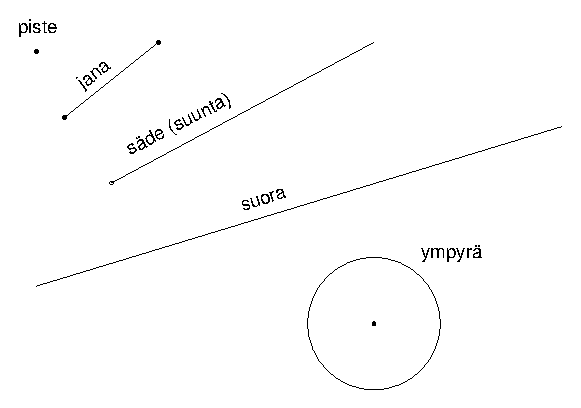
\epsfig{file=kuvat/kuvaII-1.eps}
\end{center}
%\caption{Euklidisen tason olioita}
\label{fig:oliot}
\end{figure}

Sellaiset geometriset operaatiot kuin yhdensuuntaisten suorien piirtäminen, suoran kulman
konstruoiminen, tai annetun geometrisen olion (pistejoukon) \kor{siirto} ja \kor{kierto}
\index{euklidinen liike}%
eli nk.\ \kor{euklidinen liike} (esim.\ janan siirtely pituus säilyttäen) tapahtuvat
euklidisessa geometriassa ympyräviivojen (käytännössä harpin) avulla. Myös suora on 
konstruoitavissa pelkästään harppia käyttäen, sillä suora on sellaisten pisteiden joukko
eli \kor{ura}, jotka ovat yhtä etäällä kahdesta annetusta pisteestä. --- Viivoitinta 
tarvitaan geometriassa siis vain pisteiden 'massatuotantovälineenä'. 

\subsection*{Kulma}
\index{kulma|vahv}%

Kulman määrittelee geometriassa kaksi suuntaa. Konkreettisemmin kulma on ajateltavissa
pistejoukoksi, jonka muodostavat kaksi samasta pisteestä lähtevää puolisuoraa, tai
vaihtoehtoisesti näiden puolisuorien rajaamaksi euklidisen tason \kor{sektoriksi}.
Jälkimmäisessä tulkinnassa (ei edellisessä!) on tehtävä ero \kor{sisäkulman} ja 
\kor{ulkokulman} välillä. Jos $A$ ja $B$ ovat puolisuorilla olevia pisteitä ja $O$ on 
puolisuorien yhteinen piste eli kulman \kor{kärki} ($A \neq O$, $B \neq O$), niin kulma
merkitään $\kulma AOB$. Kuvioon on merkitty sisäkulma (sektoritulkinta!) ympyräkaarella.  
\begin{figure}[H]
\setlength{\unitlength}{1cm}
\begin{center}
\begin{picture}(6,3)(-2,0)
%\Thicklines
\put(0,0){\line(3,2){4}} \put(0,0){\line(-3,3){3}}
\put(-1.55,1.45){\line(1,1){0.1}} 
\put(2.7,1.8){\line(-2,3){0.04}} \put(2.7,1.8){\line(2,-3){0.04}}
\put(-0.1,-0.5){$O$} \put(2.75,1.4){$A$} \put(-1.85,1.05){$B$}
\put(0,0){\arc{1}{-2.356}{-0.61}}
\end{picture}
\end{center}
\end{figure}
Kulmien vertailussa ja laskuoperaatioissa (myös kulman mittauksessa jäljempänä) tulkitaan
kulma yleensä sektoriksi. Sanotaan tällöin, että kaksi kulmaa ovat \kor{yhtä suuret}, jos
ne voidaan muuntaa toisikseen euklidisella liikkeellä.\footnote[2]{Kulmien yhtäsuuruus on
kulmien joukossa määritelty ekvivalenssirelaatio, vrt.\ Luku \ref{logiikka}.} 
Yhtäsuuruus on siis tarkistettavissa geometrisesti. Myös kahden kulman \kor{summa} ja 
\kor{erotus} voidaan määrätä geometrisesti siirtämällä toista kulmaa euklidisella liikkeellä
niin, että kulmat joutuvat 'vierekkäin' (summa) tai 'päällekkäin' (erotus). Geometrisella
yhteenlaskulla on esimerkiksi todistettavissa tunnettu kolmion kulmia koskeva väittämä: 
Kulmien summa = \kor{oikokulma} (Harj.teht.\,\ref{H-II-1: kulmat}b).

Jos kahdessa kolmiossa (vastin)kulmat ovat yhtä suuret, niin kolmiot ovat
\index{kulma!a@yhdenmuotoisuus} \index{yhdenmuotoisuus}%
\kor{yhdenmuotoiset}. Geometrian perusväittämiin kuuluu, että yhdenmuotoisissa kolmioissa
vastinsivujen pituuksien suhteet ovat samat. Väittämä näyttelee keskeistä roolia monissa
geometrisissa todistuksissa (ks.\ esim.\ Harj.teht.\,\ref{H-II-1: yhdenmuotoisuus}). 

\subsection*{Geometriset luvut}
\index{geometrinen luku|vahv}%
\index{laskuoperaatiot!ba@geometristen lukujen|vahv}

Kulmien mittalukuja ei euklidisen geometrian perusoperaatioissa tarvita. Sen sijaan janan 
pituuden mittaus harpin ja mittajanan avulla on perusgeometriaa. Operaatio tuo geometriaan 
reaaliluvut (tai ainakin osan niistä) ja myös lukuihin liittyvät laskutoimitukset.
Lähtökohtana pidetään lukuja $0$ ja $1$:
\[
0\ \vast\ \text{piste}, \quad 1\ \vast\ \text{mittajana}.
\]
Kun tarkastellaan kiinteää suoraa, jolta valitaan referenssipiste $O$ luvun $0$ vastineeksi, 
niin kahden (janan pituutena) annetun luvun summa ja erotus voidaan määrätä geometrisesti:
\begin{figure}[htb]
\begin{center}
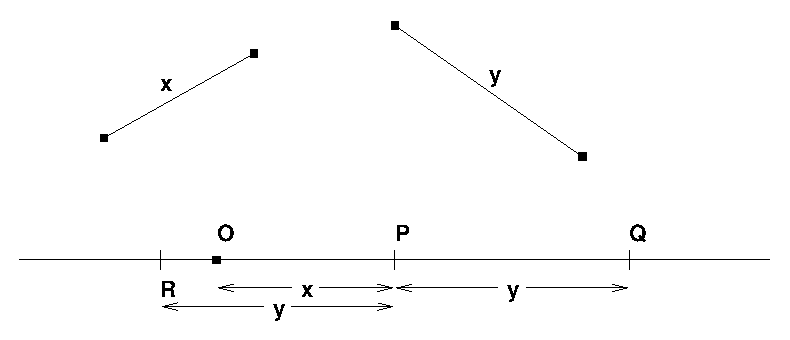
\epsfig{file=kuvat/kuvaII-2.eps}
\end{center}
%\caption{Kahden janan pituuksien summa ja erotus}
%\label{fig:summajaerotus}
\end{figure}

Kuvassa summalla ja erotuksella on geometriset vastineet janoina ja suoran pisteinä:
\begin{align*}
\qquad &x+y\ \vast\ OQ\ \vast Q,  \\
\qquad &x-y\ \vast\ OR\ \vast R.
\end{align*}
Kun janan loppupiste on $O$:sta vasemmalle (suuntahan oli määritelty!), voidaan $OR$ tulkita 
negatiiviseksi luvuksi $x-y$. Näin on siis lukujärjestelmässä määritelty sekä yhteenlasku että
vähennyslasku. Kun sääntöjä $+,-$ sovelletaan peräkkäin lähtien luvusta 1 (= mittajana
sijoitettuna suoralle) nähdään, että minkä tahansa kokonaisluvun $m\in{\Z}$ geometrinen vastine
saadaan äärellisellä määrällä geometrisia operaatioita. Siis {\Z} on konstruoitu geometrisesti.
Myös millä tahansa kokonaisluvulla jakaminen onnistuu 'viipaloimalla' luku yhdensuuntaisilla 
suorilla, joita voidaan \pain{tasossa} tuottaa harpilla ja viivoittimella (ks.\ kuvio alla).
\begin{figure}[htb]
\begin{center}
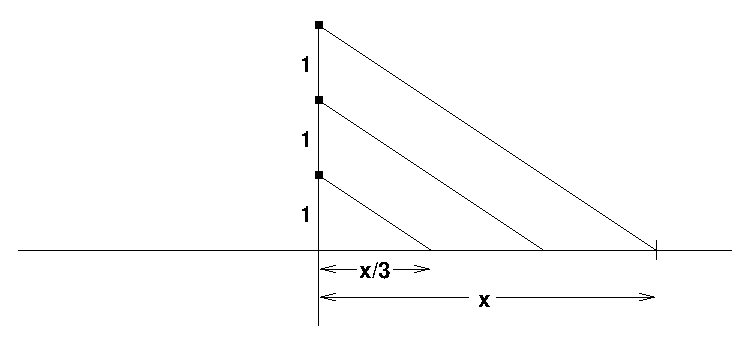
\epsfig{file=kuvat/kuvaII-3.eps}
\end{center}
\end{figure}

\pagebreak

Yleisemmin jos lähtökohtana on kaksi mittalukua $x,y$, niin niiden välinen kerto- ja jakolasku
voidaan suoraan geometrisoida yhdenmuotoisten kolmioiden avulla käyttäen suhteita 
\begin{align*}
&\frac{z}{x}\ =\ \frac{y}{1} \quad (z=xy), \\
&\frac{z}{1}\ =\ \frac{x}{y} \quad (z=x/y).
\end{align*}
Kuvassa (alla) on
\begin{alignat*}{3}
OA &\ \vast\ 1,\quad & OB &\ \vast\ y,\quad & BC&\ \vast\ OD\ \vast\ x, \\
OE &\ \vast\ x\cdot y,\quad & AF &\ \vast\ x/y. &&
\end{alignat*} 
\begin{figure}[H]
\setlength{\unitlength}{0.67cm}
\begin{center}
\begin{picture}(12,9)(-3.5,-6)
\put(-2,0){\line(1,0){11}}
\put(-0.1,-0.1){$\bullet$} \put(-0.5,0.5){$O$}
\put(2.9,-0.1){$\bullet$} \put(3,-0.6){$A$}
\put(4.9,-0.1){$\bullet$} \put(4.9,-0.6){$B$}
\put(7.9,1.9){$\bullet$} \put(7.9,2.4){$C$}
\put(4.7,1.1){$\bullet$} \put(4.3,1.4){$F$}
\put(-1.84,-3.26){$\bullet$} \put(-1.5,-3.4){$D$}
\put(-3.02,-5.4){$\bullet$} \put(-2.6,-5.5){$E$}
\put(-3,-4){\line(3,2){11}}
\put(-3.5,-5.67){\line(3,2){12.5}}
\put(-2,-0.5){\line(4,1){11}}
\path(0,0)(-3.5,-6.34)
\put(0,-0.2){$\underbrace{\hspace{2cm}}_1$}
\put(0,0.4){$\overbrace{\hspace{3.33cm}}^y$}
\put(6.8,0.8){$x$}
\put(7.2,1.1){\vector(3,2){1.15}}
\put(6.55,0.7){\vector(-3,-2){1}}
\put(-1.3,-1.6){$x$}
\put(-1.1,-1.3){\line(10,18){0.6}}
\put(-0.5,-0.25){\vector(2,3){0.13}}
\put(-1.3,-1.8){\line(-10,-19){0.6}}
\put(-1.9,-2.92){\vector(-2,-3){0.05}}
\end{picture}
\end{center}
\end{figure}
Jatkossa nimetään luvut, jotka ovat konstruoitavissa (janan pituutena) äärellisellä määrällä
geometrisia operaatioita, \kor{geometrisiksi luvuiksi}\footnote[2]{Englanninkielinen termi on 
'constructible numbers'. Suomennos ei ole vakiintunut.}, ja käytetään tälle lukujoukolle 
symbolia $\G$\,:
\begin{align*}
\G \ = \ \text{\{geometriset luvut\}}. 
\end{align*}
Tiedetään jo, että $\G$ sisältää kaikki rationaaliluvut: $\G\supset\Q$. Lisäksi tiedetään, että
$\G$ on peruslaskutoimitusten suhteen suljettu:
\[
x,y \in \G \qimpl x+y,\ x-y,\ xy,\ x/y \in \G \quad (y\neq0).
\]
Tämä merkitsee, että $(\G,+,\cdot)$ on \pain{kunta}.

Lukujoukon $\G$ muodostamisessa eivät geometrian mahdollisuudet lopu aivan 
peruslaskutoimituksiin, sillä Pythagoraan lauseen mukaan myös operaatiot
\begin{align*}
&x,y\ \map\ \sqrt{x^{2}+y^{2}}, \quad x,y \in \G, \\
&x,y\ \map\ \sqrt{x^{2}-y^{2}}, \quad x,y \in \G,\ x \ge y
\end{align*}
ovat geometrisesti toteutettavissa. Erityisesti on siis vuosituhansia päänvaivaa aiheuttanut
luku $\sqrt{2}$ geometristen lukujen joukossa:
\begin{figure}[H]
\setlength{\unitlength}{1cm}
\begin{center}
\begin{picture}(2.5,2.5)(-0.5,0)
\path(0,2)(0,0)(2,0)(0,2)
\put(0.8,-0.5){$1$} \put(-0.3,0.9){$1$} \put(0.9,1.1){$\sqrt{2}$}
\path(0.15,0)(0.15,0.15)(0,0.15)
\end{picture}
\end{center}
\end{figure}
Itse asiassa neliöjuurioperaatio $\,x\ \map\ \sqrt{x}\,$ on geometrisesti mahdollinen, olipa
mittaluku $x \in \G$ (ajatellaan $x \geq 0$) mikä tahansa:
\begin{figure}[H]
\setlength{\unitlength}{1cm}
\begin{center}
\begin{picture}(7,4.5)(0,-0.5)
\path(3,4)(0,0)(3,0)(3,4)(8.33,0)(3,0)
%\put(3,0){\arc{0.6}{-3.14}{-1.6} \linethickness{0.05cm} \put(-0.12,0.12){\picsquare}}
%\put(3,4){\arc{0.6}{0.8}{2.2} \linethickness{0.1cm} \put(0,-0.15){\picsquare}}
\path(2.85,0)(2.85,0.15)(3,0.15) %\path(2.82,3.76)(3,3.625)(3.18,3.865)
\path(2.91,3.88)(3,3.812)(3.09,3.932)
\put(0,-0.2){$\underbrace{\hspace{3cm}}_{1}$} \put(3,-0.2){$\underbrace{\hspace{5.33cm}}_{x}$}
\put(2.8,1.9){$\left. \begin{array}{c} \vspace{3.4cm} \end{array} \right\} 
                                                                    \scriptstyle{y=\sqrt{x}}$}
\end{picture}
\end{center}
\end{figure}
Tähän geometrian mahdollisuudet kuitenkin loppuvat, joten $\G$ koostuu kaikkiaan luvuista, jotka
on saatu mittaluvusta $1$ lähtien äärellisellä määrällä viittä eri operaatiota: 
$+$, $-$, $\cdot\,$, $/$ ja $\sqrt{ }\,$. Kun $\G$ vielä varustetaan geometrisella 
järjestysrelaatiolla (janojen pituuksien vertailu harpin avulla), niin tuloksena on pelkästään
geometrisiin operaatioihin perustuva järjestetty kunta $(\G,+,\cdot,<)$. Tämä on 
rationaalilukujen kunnan pienin mahdollinen laajennus, joka täyttää ehdon 
$x\in\G\,\ja\,x>0\ \impl\ \sqrt{x}\in\G$ (vrt.\ lukujoukon $\J$ konstruktio Luvussa
\ref{kunta}). On osoitettavissa, että kaikki geometriset luvut ovat algebrallisia (!), joten
pätee
\[ 
\Q\ \subset\ \G\ \subset\ \A\ \subset\ \R.
\]
Kun geometriset luvut sijoitetaan em.\ tavalla kiinteälle suoralle, voidaan näiden lukujen 
'väliin' ajatella sijoitelluksi myös muut reaaliluvut. Näin ajatellen jokainen reaaliluku saa 
geometrisen vastineen
\index{lukusuora}
\kor{lukusuoran} pisteenä.

\begin{figure}[H]
\setlength{\unitlength}{1cm}
\begin{center}
\begin{picture}(14,2)(-2,0)
\put(-1,0){\line(1,0){13}}
\put(0,0){\line(0,1){0.2}}
\put(5,0){\line(0,1){0.2}}
\put(10,0){\line(0,1){0.2}}
\put(20,0){\line(0,1){0.1}}
\put(2.07,0){\line(0,1){0.1}}
\put(8.6,0){\line(0,1){0.1}}
\put(10.7,0){\line(0,1){0.1}}
\put(2.07,1){\vector(0,-1){0.6}} \put(8.6,1){\vector(0,-1){0.6}}
\put(10.7,1){\vector(0,-1){0.6}}
\put(-0.1,-0.5){$1$} \put(4.9,-0.5){$2$} \put(9.9,-0.5){$3$}
\put(1.8,1.5){$\sqrt{2}$} \put(8.5,1.5){$e$} \put(10.6,1.5){$\pi$} 
%\multiput(0,2)(0,10){2}{\line(-1,0){0.1}}
%\multiput(0,6.5)(0,1){2}{\line(-1,0){0.1}}
%\put(-0.6,8){\vector(1,-1){0.5}}
%\put(-0.6,6){\vector(1,1){0.5}}
\end{picture}
\end{center}
\end{figure}

\subsection*{Kulman mittaluku}
\index{kulma!b@kulman mittaluku|vahv}%

Kulmien käsittelyssä geometrian mahdollisuudet ovat melko rajalliset. Kulmien yhteen- ja
vähennyslasku onnistuu geometrisesti, kuten todettiin, ja kulman voi helposti myös 
puolittaa eli jakaa kahteen yhtä suureen osaan geometrian keinoin. Sen sijaan jo kulman
jako kolmeen yhtä suureen osaan (äärellisellä) geometrisella konstruktiolla on mahdotonta,
ellei kyse ole erikoisesta (kuten suorasta) kulmasta. Geometrian keinot loppuvat myös, kun
kulmalle yritetään määrittää sen suuruutta kuvaava mittaluku. Geometrisesti pystytään 
konstruoimaan vain lukujono, jonka raja-arvo mittaluku on, eli mittaluku saadaan selville
vain päättymättömällä konstruktiolla. 
\begin{multicols}{2} \raggedcolumns
Tarkastellaan kulmaa $\kulma AOB$, missä pisteet $A$ ja $B$ on sijoitettu $O$-keskisen
\index{yksikköympyrä}%
\kor{yksikköympyrän} kehälle, ts.\ janat $OA$ ja $OB$ ovat valitun mittajanan pituiset
(vastaten lukua $1$ lukusuoralla).
\begin{figure}[H]
\setlength{\unitlength}{1cm}
\begin{center}
\begin{picture}(4.5,3.5)(-0.5,0.3)
\put(2,2){\bigcircle{4}}
\put(2,2){\line(3,1){1.9}}
\put(2,2){\line(1,3){0.63}}
\put(1.9,1.5){$O$} \put(4,2.55){$A$} \put(2.55,4){$B$}
\end{picture}
\end{center}
\end{figure}
\end{multicols}
Kuvion tilanteessa asetetaan kulman $\kulma AOB$ mittaluvuksi yksikköympyrän
\kor{kaarenpituus} pisteiden $A$ ja $B$ välillä. Koska vaihtoehtoja on kaksi, on
päätettävä, mitataanko sisä- vai ulkokulmaa. Seuraavaksi on ratkaistava vakavampi ongelma:
Miten määritellä ympyräkaaren pituus? Seuraavassa ongelman ratkaisussa yhdistellään
geometrian ja algebran keinoja.

Koska kulman $\kulma OAB$ puolitus onnistuu geometrisesti, niin saman tien kulma on
jaettavissa $n=2^k$ yhtä suureen osaan jokaisella $k\in\N$. Olkoon $k\in\N$ annettu
ja merkitään jaossa syntyviä osakulmia $\kulma P_{i-1} O P_i,\ i=1 \ldots n=2^k$,
missä $P_0=A$, $P_n=B$ ja muutkin pisteet $P_i$ ovat samalla $O$-keskisellä
ympyräkaarella. Yhdistetään nyt peräkkäiset pisteet $P_i$ janoilla \kor{murtoviivaksi}
$P_0 \ldots P_n$ ja asetetaan $\,a_k=$ ko.\ murtoviivan pituus, ts.\ $\,a_k=$ janojen 
$P_{i-1}P_i,\ i=1 \ldots n\,$ pituuksien summa. On ilmeistä, että lukujonon $\seq{a_k}$
jokainen termi on määrättävissä geometrisesti lähtien  luvusta $a_0=$ janan $AB$ pituus,
jolloin on $a_k/a_0\in\G\ \forall k$ (mahdollisesti $a_0\not\in\G$). Kuviossa on
konstruoitu murtoviiva $P_0 \ldots P_n$ indekseillä $k=0,1,2$, kun mitattavana on
suora kulma.
\begin{figure}[H]
\setlength{\unitlength}{1cm}
\begin{picture}(6,4.5)(-0.3,-0.5)
\put(0,0){\line(1,0){4}}
\put(0,0){\line(0,1){4}}
\put(0,0){\arc{6}{-1.57}{0}}
\path(3,0)(0,3)
\put(3.1,0.15){$P_0$} \put(0.1,3.15){$P_1$}
\put(1,-0.8){$k=0$}
\put(5,0){\line(1,0){4}}
\put(5,0){\line(0,1){4}}
\put(5,0){\arc{6}{-1.57}{0}}
\path(8,0)(7.121,2.121)(5,3)
\path(5,0)(7.121,2.121)
\put(8.1,0.15){$P_0$} \put(5.1,3.15){$P_2$} \put(7.22,2.27){$P_1$}
\put(6,-0.8){$k=1$}
\put(10,0){\line(1,0){4}}
\put(10,0){\line(0,1){4}}
\put(10,0){\arc{6}{-1.57}{0}}
\path(13,0)(12.772,1.148)(12.121,2.121)(11.148,2.772)(10,3)
\path(10,0)(12.772,1.148) \path(10,0)(12.121,2.121) \path(10,0)(11.148,2.772)
\put(13.1,0.15){$P_0$} \put(10.1,3.15){$P_4$} \put(12.22,2.27){$P_2$}
\put(12.87,1.3){$P_1$} \put(11.25,2.92){$P_3$}
\put(11,-0.8){$k=2$}
%\dashline{0.2}(0.3,3.4)(3.3,1.4)
%\put(1.56,2.8){$P$}
%\path(2.93,0.6)(3.3,0.6)
%\path(2.08,3.1)(2.8,3.1)
\end{picture}
\end{figure}
Pythagoraan lauseeseen vedoten on helppo näyttää, että lukujono $\seq{a_k}$ on aidosti
kasvava (Harj.teht.\,\ref{H-II-1: suoran kulman mitta}a), ja geometrisin perustein on myös
osoitettavissa, että $\seq{a_k}$ on rajoitettu lukujono 
(Harj.teht.\,\ref{H-II-1: suoran kulman mitta}b). Tämän jälkeen on turvattava algebraan: 
Koska $\seq{a_k}$ siis on kasvava ja rajoitettu lukujono, niin on olemassa raja-arvo 
$\lim_k a_k=a\in\R$ (Lause \ref{monotoninen ja rajoitettu jono}, 
Määritelmä \ref{reaaliluvut desimaalilukuina}). Määritellään kaaren $AB$ pituus, eli kulman 
$\kulma AOB$ mittaluku, kyseisenä raja-arvona $a$. 

Mittayksikköä kulman kaarenpituusmittauksessa sanotaan \kor{radiaaniksi}. Tunnetusti
luku $\,\pi=3.14159..\,$ määritellään yksikköympyrän puolikkaan kaarenpituutena, eli
\[
\boxed{\kehys\quad \pi \,=\, \text{oikokulman mittaluku}. \quad}
\]
Koska $\pi$ on transkendenttinen luku (ks.\ Luku \ref{reaalilukujen ominaisuuksia}), niin
myös suoran kulman mittaluku ($=\pi/2$) on transkendenttinen, samoin esimerkiksi
tasasivuisen kolmion kulman mittaluku ($=\pi/3$).

Kulmia on perinteisesti mitattu myös \kor{asteina} ($\aste$), jolloin oikokulman mitaksi
on sovittu $180\aste$. Yleisemmin mittaluvut asteina ja radiaaneina saadaan skaalaamalla
toisistaan:
\[
\boxed{\kehys\quad \text{kulma asteina}\ 
               =\ \frac{180}{\pi}\,\cdot\,\text{(kulma radiaaneina)}. \quad}
\]

\Harj
\begin{enumerate}

\item \label{H-II-1: kulmat}
a) Suoran leikatessa kaksi yhdensuuntaista suoraa syntyy kahdeksan kulmaa. Näytä, että
näistä jokainen on yhtä suuri kolmen muun kanssa. \newline
b) Todista: Kolmion kulmien summa = oikokulma.

\item \label{H-II-1: yhdenmuotoisuus} \index{keskijana (kolmion)}
a) Jana jakaa suorakulmaisen kolmion kahteen osaan siten, että syntyy kolme yhdenmuotoista 
kolmiota. Lähtien tästä ajatuksesta ja kolmioiden yhdenmuotoisuusopista todista Pythagoraan 
lause! \newline
b) Kolmion \kor{keskijana} yhdistää kolmion kärjen vastakkaisen sivun keskipisteeseen.
Lähtien kolmioiden yhdenmuotoisuusopista todista: Kolmion $ABC$ keskijana $AD$ puolittaa
jokaisen janan $BC$ suuntaisen janan, jonka päätepisteet ovat sivuilla $AB$ ja $AC$.

\item \index{kultainen leikkaus}
Esitä geometrinen konstruktio (aseina harppi ja viivoitin), jonka tulos on \newline
a) \ ympyrä, joka kulkee annetun kolmen pisteen kautta, \newline
b) \ annetun kolmion sisään piirretty (suurin mahdollinen) ympyrä, \newline
c) \ suora, joka kulkee annetun pisteen kautta ja sivuaa annettua ympyrää,
d) \ annetun janan $AB$ \kor{kultainen leikkaus} eli janalla oleva piste $C$ siten, että
jos $a,b,c$ ovat janojen $AB$, $AC$ ja $CB$ pituudet, niin $\,a/b=b/c$.

\item
Seuraavista luvuista kaksi ei ole geometrisia. Mitkä kolme ovat\,? \vspace{1mm}\newline
a) \ $\sqrt[1024]{17}$ $\quad$ b) \ $\sqrt[3]{512}$ $\quad$ c) \ $\sqrt[6]{343}$ $\quad$
d) \ $\sqrt[3]{7\sqrt{2}+5}$ $\quad$ e) \ $\sqrt[3]{5\sqrt{2}+7}$

\item (*) \label{H-II-1: suoran kulman mitta}
Suoran kulman mittaluku radiaaneina määritellään raja-arvona $\,a=\lim_k a_k$, missä $4a_k=$ sen 
säännöllisen $2^{k+2}$-kulmion piiri, jonka kärjet ovat yksikköympyrällä. \vspace{1mm}\newline
a) Näytä, että lukujono $\seq{a_k}_{k=0}^\infty$ on aidosti kasvava. \newline
b) Näytä, että $a_k < 2\ \forall k$. \newline
c) Näytä, että $\seq{a_k}$ on laskettavissa palautuvana lukujonona
\[
a_0=\sqrt{2}, \quad 
a_{k+1}=\frac{2a_k}{\sqrt{2+\sqrt{4-(2^{-k}a_k)^2}}}\,, \quad k=0,1,\ldots
\]
Laske $a_k,\ k=1 \ldots 5$ ja vertaa lukuun $\tfrac{\pi}{2}$.

\end{enumerate}